\section{Produktfunktionen}
	% \input{3-Produktfunktionen}

		\subsection{Use Cases}
		% \input{3-1-Use_Cases}
		
		Die Abbildungen \ref{fig:3-1-robot-use-cases}, \ref{fig:3-1-server-use-cases} und \ref{fig:3-1-hospital-use-cases} zeigen die Funktionalitäten der Teilsysteme \emph{Robot}, \emph{Server} sowie \emph{Hospital}.
		
			\begin{figure}[H]
				\centering
				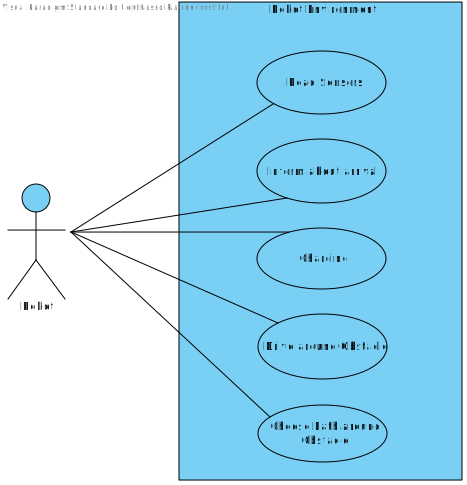
\includegraphics[width=0.8\textwidth]{img/1-Analyse-3-Robot}
				\caption{Use Case Diagramm 1: Use Cases des Robots}
				\label{fig:3-1-robot-use-cases}
			\end{figure}

			\begin{figure}[H]
				\centering
				\includegraphics[width=0.8\textwidth]{img/1-Analyse-3-Server}
				\caption{Use Case Diagramm 2: Use Cases des Servers}
				\label{fig:3-1-server-use-cases}
			\end{figure}

			\begin{figure}[H]
				\centering
				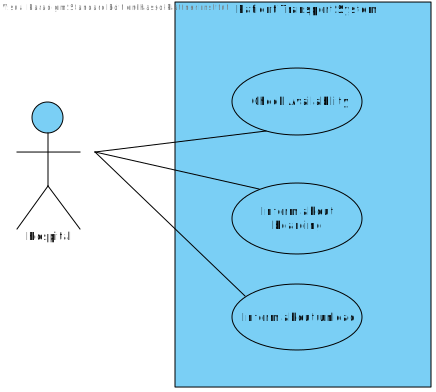
\includegraphics[width=0.8\textwidth]{img/1-Analyse-3-Hospital}
				\caption{Use Case Diagramm 2: Use Cases des Hospitals}
				\label{fig:3-1-hospital-use-cases}
			\end{figure}

		\pagebreak

		\subsection{Beschreibung zu Use Case \emph{1}: Choose Path around Obstacle}

			\subsubsection*{Charakterisierende Informationen}

			\begin{table}[H]
				\centering
				\begin{tabularx}{\textwidth}{@{}p{5cm}X@{}}
				\hline
				\textbf{Übergeordneter elementarer Geschäftsprozess:} & Drive to Destination\\ \hline
				\textbf{Ziel des Use Cases:} & \emph{Robot} wählt einen Weg um ein \emph{Obstacle} \\ \hline
				\textbf{Umgebende Systemgrenze:} & \emph{Robot} \\ \hline
				\textbf{Vorbedingung:} & Der \emph{Robot} befindet sich dabei, eine \emph{Destination} anzufahren \\ \hline
				\textbf{Nachbedingung bei erfolgreicher Ausführung:} & 
				Der \emph{Robot} umfährt das \emph{Obstacle} \\ \hline
				\textbf{Beteiligte Nutzer:} & \emph{Robot} \\ \hline
				\textbf{Auslösendes Ereignis:} & Ein \emph{Robot} hat ein \emph{Obstacle} auf dem Weg zwischen sich und der \emph{Destination} gefunden\\ \hline
				\end{tabularx}
			\end{table}

			Dieser Use Case wird dann benutzt, wenn ein \emph{Robot} auf dem Weg zu seiner aktuellen \emph{Destination} ein \emph{Obstacle} vor sich findet, das umfahren werden muss. Im Wesentlichen spricht der Robot dann seine Peripherie an, um Informationen über das \emph{Obstacle} zu sammeln. Dabei findet eine Fallunterscheidung statt, sodass sich zum Beispiel zwei gegenüberstehende \emph{Robots} erkennen und beide nach rechts ausweichen. Bei statischen \emph{Obstacles} wird diese Entscheidung abhängig von dem Teil des \emph{Obstacles} entschieden, den der \emph{Robot} mit seinen Sensoren wahrnehmen kann.
		
		\pagebreak
		
		
		\subsection{Beschreibung zu Use Case \emph{2}: Drive around Obstacle}

			\subsubsection*{Charakterisierende Informationen}

			\begin{table}[H]
				\centering
				\begin{tabularx}{\textwidth}{@{}p{5cm}X@{}}
				\hline
				\textbf{Übergeordneter elementarer Geschäftsprozess:} & Drive to Destination\\ \hline
				\textbf{Ziel des Use Cases:} & \emph{Robot} umfährt ein \emph{Obstacle} \\ \hline
				\textbf{Umgebende Systemgrenze:} & \emph{Robot} \\ \hline
				\textbf{Vorbedingung:} & Ein \emph{Robot} hat ein \emph{Obstacle} auf dem Weg zwischen sich und der \emph{Destination} gefunden\\ \hline
				\textbf{Nachbedingung bei erfolgreicher Ausführung:} & 
				Der \emph{Robot} umfährt das \emph{Obstacle} \\ \hline
				\textbf{Beteiligte Nutzer:} & \emph{Robot} \\ \hline
				\textbf{Auslösendes Ereignis:} & Der \emph{Robot} hat den besten (nach seinen Berechnungen) Weg um das \emph{Obstacle} gewählt. \\ \hline
				\end{tabularx}
			\end{table}
		Dieser Use Case beschreibt die eigentliche Umfahrung eines \emph{Obstacles} von einem \emph{Robot}. Der \emph{Robot} hat davor ausgewählt, zu welcher Richtung hin er das \emph{Obstacle} umfahren möchte. Wenn es sich um ein statisches \emph{Obstacle} handelt, fährt der \emph{Robot} immer eine kleine Distanz parallel zur Kante des \emph{Obstacles} und prüft ob der Weg zur \emph{Destination} wieder frei ist. Wenn dieser frei ist, wird die normale Fahrt wieder aufgenommen, ansonsten wird der Kurs wieder parallel zur Kante des \emph{Obstacles} korrigiert und der Vorgang wiederholt. Wenn sich zwei \emph{Robots} gegenseitig als \emph{Obstacles} wahrgenommen haben, ist ihnen aus dem Use Case \textit{Choose Path around Obstacle} klar, dass sie beide nach rechts ausweichen müssen, um dann den Normalbetrieb wieder aufzunehmen.
			
			%\subsubsection*{Beschreibung des allgemeinen Ablaufes}
			
		\pagebreak

		\subsection{Beschreibung zu Use Case \emph{3}: Read Sensors}

			\subsubsection*{Charakterisierende Informationen}

			\begin{table}[H]
				\centering
				\begin{tabularx}{\textwidth}{@{}p{5cm}X@{}}
				\hline
				\textbf{Übergeordneter elementarer Geschäftsprozess:} & Choose Robot\\ \hline
				\textbf{Ziel des Use Cases:} & \emph{Robot} kann über seinen Akkustand und seine Position Auskunft geben\\ \hline
				\textbf{Umgebende Systemgrenze:} & \emph{Robot} \\ \hline
				\textbf{Vorbedingung:} & \emph{Robot} hat eine Anfrage vom \emph{Server} erhalten \\ \hline
				\textbf{Nachbedingung bei erfolgreicher Ausführung:} & \emph{Robot} schickt die ermittelten Informationen an den \emph{Server} \\ \hline
				\textbf{Beteiligte Nutzer:} & \emph{Robot} \\ \hline
				\textbf{Auslösendes Ereignis:} & \emph{Robot} hat eine Anfrage vom \emph{Server} erhalten, seine Sensoren zu lesen und sie dem \emph{Server} zu schicken \\
				\hline
				\end{tabularx}
			\end{table}

			Im Rahmen vom Geschäftsprozess \emph{Choose Robot} sammelt der \emph{Server}
			Informationen über jeden \emph{Robot}. Diese Informationen (z.B
			Akkustand, aktuelle Position, ob der \emph{Robot} gerade ein Ziel verfolgt)
			kann der \emph{Robot} von seinen Hardware-Schnittstellen anfordern. Dieses
			Use Case wird dann ausgefüht, wenn der \emph{Robot} eine Anfrage vom
			Server erhält, seine Sensoren zu lesen, und endet damit, dass der \emph{Robot}
			die zusammengefassten Informationen an den \emph{Server} schickt.

			\subsubsection*{Szenario für den Standardablauf (Erfolg)}

			\begin{table}[H]
				\centering
				\begin{tabularx}{\textwidth}{@{}cp{2cm}X@{}}
				\hline
				Schritt & Nutzer & Beschreibung der Aktivität \\ \hline
				1 & Robot & \emph{Robot} erhält Anfrage vom \emph{Server} \\
				2 & Robot & \emph{Robot} sammelt Informationen von seiner Hardwareschnittstelle und fasst sie zusammen \\
				3 & Robot & \emph{Robot} schickt zusammengefasste Informationen an den Server \\
				\hline
				\end{tabularx}
			\end{table}

			%\subsubsection*{Beschreibung des allgemeinen Ablaufes}
			
		\pagebreak

		\subsection{Beschreibung zu Use Case \emph{4}: Charging}

			\subsubsection*{Charakterisierende Informationen}

			\begin{table}[H]
				\centering
				\begin{tabularx}{\textwidth}{@{}p{5cm}X@{}}
				\hline
				\textbf{Übergeordneter elementarer Geschäftsprozess:} & Drive to Destination\\ \hline
				\textbf{Ziel des Use Cases:} & Ziel ist es, dem \emph{Robot} zu ermöglichen seine Ladestation anzufahren\\ \hline
				\textbf{Umgebende Systemgrenze:} & \emph{Robot}\\ \hline
				\textbf{Vorbedingung:} & Der \emph{Robot} erreicht sein vorgegebenes Ziel\\ \hline
				\textbf{Nachbedingung bei erfolgreicher Ausführung:} & Der \emph{Robot} erreicht seine Ladestation\\ \hline
				\textbf{Beteiligte Nutzer:} & \emph{Robot}\\ \hline
				\textbf{Auslösendes Ereignis:} & \emph{Robot} erreicht \emph{Destination} (Use-Case)\\
				\hline
				\end{tabularx}
			\end{table}

			Jedem Robot wird, laut Aufgabenstellung, eine feste Ladestation zugewiesen. Der Robot fährt vollständig autonom diese Ladestation an. Daher ist keine Kommunikation mit dem Server notwendig.

			\subsubsection*{Szenario für den Standardablauf (Erfolg)}

			\begin{table}[H]
				\centering
				\begin{tabularx}{\textwidth}{@{}cp{2cm}X@{}}
				\hline
				Schritt & Nutzer & Beschreibung der Aktivität \\ \hline
				1 & Robot & \emph{Robot} erreicht Ziel \\
				2 & Robot & \emph{Robot} fährt zur Ladestation \\
				3 & Robot & \emph{Robot} erreicht Ladestation und lädt sich auf \\
				4 & Robot & \emph{Robot} erhält neues Ziel und fährt dorthin \\
				\hline
				\end{tabularx}
			\end{table}

			%\subsubsection*{Beschreibung des allgemeinen Ablaufes}
			
		\pagebreak
		
			\subsection{Beschreibung zu Use Case \emph{5}: Inform about arrival}

			\subsubsection*{Charakterisierende Informationen}

			\begin{table}[H]
				\centering
				\begin{tabularx}{\textwidth}{@{}p{5cm}X@{}}
				\hline
				\textbf{Übergeordneter elementarer Geschäftsprozess:} & TakePatientToHospital\\ \hline
				\textbf{Ziel des Use Cases:} & Ziel ist es, dem \emph{Robot} zu ermöglichen seine Ankunft dem Krnakenhaus mitzuteilen\\ \hline
				\textbf{Umgebende Systemgrenze:} & \emph{Robot}\\ \hline
				\textbf{Vorbedingung:} & Der \emph{Robot} erreicht die \emph{Position} des Patienten\\ \hline
				\textbf{Nachbedingung bei erfolgreicher Ausführung:} & Der \emph{Robot} wartet, bis er beladen wurde\\ \hline
				\textbf{Beteiligte Nutzer:} & \emph{Robot}\\ \hline
				\textbf{Auslösendes Ereignis:} & \emph{Robot} erreicht Patienten\\
				\hline
				\end{tabularx}
			\end{table}

			Der \emph{Robot} erreicht seine vorgegebene \emph{Destination} und muss dem \emph{Hospital} mitteilen, dass er angekommen ist. 

			\subsubsection*{Szenario für den Standardablauf (Erfolg)}

			\begin{table}[H]
				\centering
				\begin{tabularx}{\textwidth}{@{}cp{2cm}X@{}}
				\hline
				Schritt & Nutzer & Beschreibung der Aktivität \\ \hline
				1 & Robot & \emph{Robot} informiert \emph{Server}, dass er angekommen ist. \\
				\hline
				\end{tabularx}
			\end{table}

			%\subsubsection*{Beschreibung des allgemeinen Ablaufes}
			
		\pagebreak

		\subsection{Beschreibung zu Use Case \emph{6}: Select best Match}

			\subsubsection*{Charakterisierende Informationen}

			\begin{table}[H]
				\centering
				\begin{tabularx}{\textwidth}{@{}p{5cm}X@{}}
				\hline
				\textbf{Übergeordneter elementarer Geschäftsprozess:} & Choose Robot \\ \hline
				\textbf{Ziel des Use Cases:} & Passenden \emph{Robot} für die aktuelle \emph{Destination} auswählen\\ \hline
				\textbf{Umgebende Systemgrenze:} & \emph{Robot} und \emph{Server} \\ \hline
				\textbf{Vorbedingung:} & \emph{Server} sucht \emph{Robot} für eine neu erhaltene \emph{Destination}\\ \hline
				\textbf{Nachbedingung bei erfolgreicher Ausführung:} & Wenn es einen geeigneten \emph{Robot} gibt, dann wird diesem die \emph{Destination} zugeteilt.\\ \hline
				\textbf{Beteiligte Nutzer:} & \emph{Robot} und \emph{Server}\\ \hline
				\textbf{Auslösendes Ereignis:} & \emph{Server} hat von allen \emph{Robots} die Sensordaten empfangen\\
				\hline
				\end{tabularx}
			\end{table}

			\subsubsection*{Szenario für den Standardablauf (Erfolg)}

			\begin{table}[H]
				\centering
				\begin{tabularx}{\textwidth}{@{}cp{2cm}X@{}}
				\hline
				Schritt & Nutzer & Beschreibung der Aktivität \\ \hline
				1 & Server & \emph{Server} erhält Sensordaten von allen \emph{Robots} \\
				2 & Server & \emph{Server} berechnet, ob es einen \emph{Robot} gibt, der zur \emph{Destination} fahren kann\\
				3 & Server & Wenn es keinen geeigneten \emph{Robot} gibt, weise die \emph{Destination} ab. \\
				4 & Server & Es gitb einen geeigneten \emph{Robot} und \emph{Server} führt den Use-Case \textit{Assign Task} aus und gibt dem \emph{Robot} die \emph{Destination}\\
				\hline
				\end{tabularx}
			\end{table}

			%\subsubsection*{Beschreibung des allgemeinen Ablaufes}
			
		\pagebreak

		\subsection{Beschreibung zu Use Case \emph{7}: Assign Task}

			\subsubsection*{Charakterisierende Informationen}

			\begin{table}[H]
				\centering
				\begin{tabularx}{\textwidth}{@{}p{5cm}X@{}}
				\hline
				\textbf{Übergeordneter elementarer Geschäftsprozess:} & Choose Robot  \\ \hline
				\textbf{Ziel des Use Cases:} & \emph{Robot} den Task (die \emph{Destination}) zuweisen\\ \hline
				\textbf{Umgebende Systemgrenze:} & \emph{Server} und \emph{Robot} \\ \hline
				\textbf{Vorbedingung:} & „Choose Robot“ hat den am besten geeigneten \emph{Robot} gefunden und ausgewählt\\ \hline
				\textbf{Nachbedingung bei erfolgreicher Ausführung:} & Ausgewählter \emph{Robot} steuert die \emph{Destination} an\\ \hline
				\textbf{Beteiligte Nutzer:} & \emph{Server} und \emph{Robot}\\ \hline
				\textbf{Auslösendes Ereignis:} & Im Use-Case „choose Robot“ wurde passender \emph{Robot} ausgewählt\\
				\hline
				\end{tabularx}
			\end{table}
			
			Dem \emph{Server} wird hiermit die Möglichkeit gegeben, dem \emph{Robot} eine beliebige \emph{Destination} zuzuweisen. 

			\subsubsection*{Szenario für den Standardablauf (Erfolg)}

			\begin{table}[H]
				\centering
				\begin{tabularx}{\textwidth}{@{}cp{2cm}X@{}}
				\hline
				Schritt & Nutzer & Beschreibung der Aktivität \\ \hline
				1 & Server & \emph{Server} überträgt ausgewähltem \emph{Robot} den Task \\
				\hline
				\end{tabularx}
			\end{table}

			%\subsubsection*{Beschreibung des allgemeinen Ablaufes}

	\pagebreak


		\subsection{Beschreibung zu Use Case \emph{8}: Check availability}

			\subsubsection*{Charakterisierende Informationen}

			\begin{table}[H]
				\centering
				\begin{tabularx}{\textwidth}{@{}p{5cm}X@{}}
				\hline
				\textbf{Übergeordneter elementarer Geschäftsprozess:} & TakePatientToHospital  \\ \hline
				\textbf{Ziel des Use Cases:} & \emph{Hospital} erfährt, ob ein Auftrag vom System entgegengenommen werden kann. \\ \hline
				\textbf{Umgebende Systemgrenze:} & \emph{Hospital} und \emph{Server} \\ \hline
				\textbf{Vorbedingung:} & Das \emph{Hospital} hat einen neuen Patienten registriert. \\ \hline
				\textbf{Nachbedingung bei erfolgreicher Ausführung:} & Das System führt den Auftrag aus und bringt den \emph{Patient} in das \emph{Hospital} \\ \hline
				\textbf{Beteiligte Nutzer:} & \emph{Hospital} und \emph{Server}\\ \hline
				\textbf{Auslösendes Ereignis:} & \emph{Hospital} hat einen neuen Auftrag\\
				\hline
				\end{tabularx}
			\end{table}

			Das \emph{Hospital} fragt laut Aufgabenstellung an dem zu modellierenden System an, ob ein \emph{Robot} verfügbar ist, um einen \emph{Patient} anzufahren und ins \emph{Hospital} zu bringen. Dazu wird vom \emph{Server} unter anderem der Use Case \emph{Choose Robot} ausgeführt. Es kann passieren, dass kein \emph{Robot} verfügbar ist, dann soll wie in der Aufgabenstellung beschrieben der Auftrag vom System abgelehnt werden. Was das \emph{Hospital} dann für Maßnahmen ergreift, wird hier nicht modelliert da es nicht teil des Systems ist.

			%\subsubsection*{Beschreibung des allgemeinen Ablaufes}

	\pagebreak
		\subsection{Beschreibung zu Use Case \emph{9}: Inform about boarding}

			\subsubsection*{Charakterisierende Informationen}

			\begin{table}[H]
				\centering
				\begin{tabularx}{\textwidth}{@{}p{5cm}X@{}}
				\hline
				\textbf{Übergeordneter elementarer Geschäftsprozess:} & TakePatientToHospital   \\ \hline
				\textbf{Ziel des Use Cases:} & Dem \emph{Robot} mitteilen, dass Patient auf den \emph{Robot} beladen wurde \\ \hline
				\textbf{Umgebende Systemgrenze:} & \emph{Hospital} \\ \hline
				\textbf{Vorbedingung:} & Patient befindet sich auf \emph{Robot}\\ \hline
				\textbf{Nachbedingung bei erfolgreicher Ausführung:} & \emph{Robot} fährt Patienten zum \emph{Hospital} \\ \hline
				\textbf{Beteiligte Nutzer:} & \emph{Hospital}\\ \hline
				\textbf{Auslösendes Ereignis:} & \emph{Server} wurde informiert, dass \emph{Robot} am Patienten angekommen ist(Inform about arrival)\\
				\hline
				\end{tabularx}
			\end{table}
			
			Das \emph{Hospital} muss dem \emph{Robot} mitteilen, dass der Patient beladen wurde um einen sicheren Transport des Patienten zu gewährleisten. Der \emph{Robot} hat somit keinen Eingriff in das Beladen des Patienten.

			\subsubsection*{Szenario für den Standardablauf (Erfolg)}

			\begin{table}[H]
				\centering
				\begin{tabularx}{\textwidth}{@{}cp{2cm}X@{}}
				\hline
				Schritt & Nutzer & Beschreibung der Aktivität \\ \hline
				1 & \emph{Hospital} & Patient wird auf Roboter beladen \\
				2 & \emph{Hospital} & \emph{Hospital} sendet Nachricht an Server, dass sich Patient auf dem \emph{Robot} befindet \\
				\hline
				\end{tabularx}
			\end{table}

			%\subsubsection*{Beschreibung des allgemeinen Ablaufes}

	\pagebreak
